\documentclass[10pt]{exam}
\printanswers
\usepackage{epsfig,amssymb}
\usepackage{xcolor}
\definecolor{darkred}{rgb}{0.5,0,0}
\definecolor{darkgreen}{rgb}{0,0.5,0}
\usepackage{hyperref}
\usepackage{fullpage}
\usepackage{tikz}
\pagestyle{empty} 
\usepackage{listings}
\setlength{\parindent}{0pt} %
\setlength{\parskip}{.25cm}
\newcommand{\comment}[1]{}
\boxedpoints
\addpoints
\usepackage{amsmath}
\usepackage{algorithm2e}
\usepackage{url}
\usepackage{enumitem}
\usepackage{graphics}

\pagestyle{headandfoot}
\firstpageheader{\Large CSCE 235}{{\Large Assignment 4}}{\Large Spring 2026}

\begin{document}

\hrule

\vspace{.50cm} Name:
\text{Charlie Pyle} 
\\ NUID: 22821006
\vspace{.50cm}

\textbf{Instructions} Follow instructions \emph{carefully}, failure to do so will result in points being deducted. Be sure to show sufficient work to justify your answer(s).

\begin{questions}

\question[12] For each of these relations on the set $\{$ants, bees, crickets, dragonflies$\}$, decide whether it is reflexive, symmetric, antisymmetric, and/or transitive. \textbf{Justify} your answer.

\begin{parts}
\part $\{$(bees, bees), (bees, crickets), (bees, dragonflies), (crickets, bees), (crickets, crickets), (crickets, dragonflies)$\}$
\part $\{$(ants, ants), (ants, bees), (bees, ants), (bees, bees), (crickets, crickets), (dragonflies, ants), (dragonflies, dragonflies)$\}$
\part $\{$(ants, ants), (bees, bees), (crickets, crickets), (dragonflies, dragonflies)$\}$
\end{parts}

\begin{solution}
    Enter your solution here:\\
    Let $A = \text{ants}$, $B = \text{bees}$, $C = \text{crickets}$, $D = \text{dragonflies}$.\\
    \textbf{A:}\\
    $R_1 = \{(B,B), (B,C), (B,D), (C,B), (C,C), (C,D)\}$\\
    \textbf{Reflexive:} No, missing $(A,A)$ and $(D,D)$.\\
    \textbf{Symmetric:} No, we have $(B,D) \in R_1$ but $(D,B) \notin R_1$.\\
    \textbf{Antisymmetric:} No, we have $(B,C) \in R_1$ and $(C,B) \in R_1$.\\
    \textbf{Transitive:} Yes, checking all required pairs:
    \begin{itemize}
        \item $(B,B)$ and $(B,C)$ implies $(B,C) \checkmark$
        \item $(B,B)$ and $(B,D)$ implies $(B,D) \checkmark$
        \item $(B,C)$ and $(C,B)$ implies $(B,B) \checkmark$
        \item $(B,C)$ and $(C,C)$ implies $(B,C) \checkmark$
        \item $(B,C)$ and $(C,D)$ implies $(B,D) \checkmark$
        \item $(C,B)$ and $(B,B)$ implies $(C,B) \checkmark$
        \item $(C,B)$ and $(B,C)$ implies $(C,C) \checkmark$
        \item $(C,B)$ and $(B,D)$ implies $(C,D) \checkmark$
        \item $(C,C)$ and $(C,B)$ implies $(C,B) \checkmark$
        \item $(C,C)$ and $(C,D)$ implies $(C,D) \checkmark$
    \end{itemize}
    All required pairs are present.\\
    
    \textbf{B:}\\
    $R_2 = \{(A,A), (A,B), (B,A), (B,B), (C,C), (D,A), (D,D)\}$\\
    \textbf{Reflexive:} Yes, contains all pairs $(x,x)$ for every element $x$ in the set.\\
    \textbf{Symmetric:} No, we have $(D,A) \in R_2$ but $(A,D) \notin R_2$.\\
    \textbf{Antisymmetric:} No, we have $(A,B) \in R_2$ and $(B,A) \in R_2$.\\
    \textbf{Transitive:} No, we have $(D,A) \in R_2$ and $(A,B) \in R_2$, but $(D,B) \notin R_2$.\\
    
    \textbf{C:}\\
    $R_3 = \{(A,A), (B,B), (C,C), (D,D)\}$\\
    \textbf{Reflexive:} Yes, contains all pairs $(x,x)$ for every element $x$ in the set.\\
    \textbf{Symmetric:} Yes, for every $(x,y) \in R_3$, we have $x = y$, so $(y,x) = (x,x) \in R_3$.\\
    \textbf{Antisymmetric:} Yes, for any $(x,y), (y,x) \in R_3$ with $x \neq y$, there are no such pairs since all pairs have the form $(x,x)$.\\
    \textbf{Transitive:} Yes, this relation contains only pairs where an element is related to itself.
\end{solution}

\question[12] Determine whether the relation R on the set of all integers is reflexive, symmetric, antisymmetric, and/or transitive, where $(x,y) \in R$ if and only if

\begin{parts}
\part $y = x $.
\part $y = x^2$. 
\part $y < x^2$.
\end{parts}

\textbf{Justify} your answer.
\begin{solution}
    Enter your solution here:\\
    \textbf{A:}\\
    \textbf{Reflexive:} For $(x,x)$ to be in $R$, we need x = x which is always true.\\
    \textbf{Symmetric:} Suppose $(x, y) \in R$, then $y = x$. For $(y, x) \in R$, we need $x = y$, which is true since $y = x$.\\
    \textbf{Antisymmetric:} Yes, for any $(x,y), (y,x) \in R$ with $x \neq y$, there are no such pairs since all pairs have the form $(x,x)$.\\
    \textbf{Transitive:} Yes, this relation contains only pairs where an element is related to itself.\\   
    
    \textbf{B:}\\
    \textbf{Reflexive:} For $(x,x)$ to be in R, we need $x = x^2$ which means $x^2 -x = 0$. This only true for $x = 0$ or $x = 1$.\\
    Counterexample: $(2,2) \notin R$ because $2 \neq 2^2$ since $2^2 = 4$, therefore $R$ is not reflexive.\\
    \textbf{Symmetric:} Suppose $(x,y) \in R$ and $(y,x) \in R$. From $(x,y) \in R$: $y = x^2$. From $(y,x) \in R$: $x = y^2 = (x^2)^2 = x^4$. This is only true when $x^4 = x^2$, i.e., $x \in \{0, 1, -1\}$.\\
    Counterexample: $(2,4) \in R$(since $4 = 2^2$, but $(4,2) \notin R$(since $2 \neq (4^2 = 16)$, therefore $R$ is not symmetric.\\
    \textbf{Antisymmetric:} Suppose $(x,y) \in R$ and $(y,x) \in R$. From $(x,y) \in R$: $y = x^2$. From $(y,x) \in R$: $x = y^2 = (x^2)^2 = x^4$.
    From $x = x^4$, we get $x^4 - x = 0$, so $x(x^3 - 1) = 0$, giving $x \in \{0, 1, -1\}$.
    If $x = 0$: then $y = 0^2 = 0$, so $x = y$. If $x = 1$: then $y = 1^2 = 1$, so $x = y$. If $x = -1$: then $y = (-1)^2 = 1$, but for $(1,-1) \in R$ we need $-1 = 1^2 = 1$, which is false. So $(1,-1) \notin R$, therefore $R$ is antisymmetric.\\
    \textbf{Transitive:} Suppose $(x,y) \in R$ and $(y,z) \in R$. From $(x,y) \in R$: $y = x^2$. From $(y,z) \in R$: $z = y^2 = (x^2)^2 = x^4$.
    For $(x,z) \in R$, we need $z = x^2$, but we have $z = x^4$. This is only true when $x^4 = x^2$, i.e., $x \in \{0, 1, -1\}$.\\
    Counterexample: $(2,4) \in R$ and $(4,16) \in R$, but $(2,16) \notin R$ since $16 \neq 2^2 = 4$, therefore $R$ is not transitive.\\
    
    \textbf{C:}\\
    \textbf{Reflexive:} For $(x,x) \in R$, we need $x < x^2$, which means $x^2 - x > 0$, so $x(x-1) > 0$.
    This is true when $x < 0$ or $x > 1$.\\
    Counterexample: $(0,0) \notin R$ because $0 \not< 0^2 = 0$, therefore $R$ is not reflexive.\\
    
    \textbf{Symmetric:} Suppose $(x,y) \in R$, so $y < x^2$.
    For $(y,x) \in R$, we need $x < y^2$.\\
    Counterexample: $(2,1) \in R$ since $1 < 2^2 = 4$, but $(1,2) \notin R$ since $2 \not< 1^2 = 1$, therefore $R$ is not symmetric.\\
    
    \textbf{Antisymmetric:} Suppose $(x,y) \in R$ and $(y,x) \in R$, so $y < x^2$ and $x < y^2$.
    From $x < y^2$, we get $x^2 < y^4$. Combined with $y < x^2$, we have $y < x^2 < y^4$.
    This gives $y < y^4$, so $y^4 - y > 0$, meaning $y(y-1)(y^2+y+1) > 0$.
    Similarly, from $y < x^2$, we get $y^2 < x^4$, and with $x < y^2$, we have $x < y^2 < x^4$.
    If $x \neq y$, these conditions cannot be satisfied simultaneously, therefore $R$ is antisymmetric.\\
    
    \textbf{Transitive:} Suppose $(x,y) \in R$ and $(y,z) \in R$. Then $y < x^2$ and $z < y^2$.
    For $(x,z) \in R$, we need $z < x^2$.
    We have $z < y^2 < (x^2)^2 = x^4$, so $z < x^4$, but this doesn't guarantee $z < x^2$.\\
    Counterexample: $(2,3) \in R$ (since $3 < 4$) and $(3,8) \in R$ (since $8 < 9$), but $(2,8) \notin R$ since $8 \not< 2^2 = 4$, therefore $R$ is not transitive.\\
\end{solution}

\question[6] Represent each of these relations on $\{A, B, C, D\}$ with a matrix (with the elements of this set listed in increasing
order).
\begin{parts}
\part $\{(A, A), (A, B), (B, C), (B, D), (C, C), (C, D), (D, D), (D, A)\}$
\part $\{(A, A), (A, D), (B, B), (B, C), (C, B), (C, C), (D, A), (D, D)\}$
\end{parts}

\begin{solution}
    Enter your solution here:\\
    \textbf{A:}\\
    \[
    \begin{bmatrix}
        1 & 1 & 0 & 0 \\
        0 & 0 & 1 & 1 \\
        0 & 0 & 1 & 1 \\
        1 & 0 & 0 & 1
    \end{bmatrix}
    \]
    \textbf{B:}\\
    \[
    \begin{bmatrix}
        1 & 0 & 0 & 1 \\
        0 & 1 & 1 & 0 \\
        0 & 1 & 1 & 0 \\
        1 & 0 & 0 & 1
    \end{bmatrix}
    \]
\end{solution}

\question[6] Consider the set $\{1, 2, 3, 4\}$. Find the transitive closure on this set of the relation $$\{(1, 1), (1, 4), (2, 1), (2, 3), (3, 1), (3,2), (3,4), (4,1), (4,3)\}$$ using Warshall's algorithm. \textbf{You must show the steps of your calculation}.

\begin{solution}
    Enter your solution here:\\
    \textbf{Initial Matrix:}
    \[W_0 = \begin{bmatrix}
    1 & 0 & 0 & 1 \\
    1 & 0 & 1 & 0 \\
    1 & 1 & 0 & 1 \\
    1 & 0 & 1 & 0
    \end{bmatrix}\]
    \textbf{Step } $k = 1$:\\
    \[W_1 = \begin{bmatrix}
    1 & 0 & 0 & 1 \\
    1 & 0 & 1 & 1 \\
    1 & 1 & 0 & 1 \\
    1 & 0 & 1 & 1
    \end{bmatrix}\]
    \textbf{Step } $k = 2$:\\
    \[W_2 = \begin{bmatrix}
    1 & 0 & 0 & 1 \\
    1 & 0 & 1 & 1 \\
    1 & 1 & 1 & 1 \\
    1 & 0 & 1 & 1
    \end{bmatrix}\]
    \textbf{Step } $k = 3$:\\
    \[W_3 = \begin{bmatrix}
    1 & 0 & 0 & 1 \\
    1 & 1 & 1 & 1 \\
    1 & 1 & 1 & 1 \\
    1 & 1 & 1 & 1
    \end{bmatrix}\]
    \textbf{Step } $k = 4$:\\
    \[W_4 = \begin{bmatrix}
    1 & 1 & 1 & 1 \\
    1 & 1 & 1 & 1 \\
    1 & 1 & 1 & 1 \\
    1 & 1 & 1 & 1
    \end{bmatrix}\]
    \textbf{Final Transitive Closure:}
    \[W^* = \begin{bmatrix}
    1 & 1 & 1 & 1 \\
    1 & 1 & 1 & 1 \\
    1 & 1 & 1 & 1 \\
    1 & 1 & 1 & 1
    \end{bmatrix}\]
\end{solution}

\question[6] Which of these relations on the set of all people are equivalence relations? Determine the properties of an equivalence relation that the others lack. \textbf{Justify} your answer.

\begin{enumerate}
 \item[(a)] $\{(a, b) |$ a and b have eaten breakfast together$\}$
 \item[(b)] $\{(a, b) |$ a and b share a common last name$\}$
\end{enumerate}

\begin{solution}
    Enter your solution here:\\
    \textbf{A:}\\
    The relation "a and b have eaten breakfast together" is:\\
    \textbf{Reflexive} - Yes: Everyone has eaten breakfast with themselves\\
    \textbf{Symmetric} - Yes: If a ate with b, then b ate with a\\
    \textbf{Transitive} - No: a eating with b and b eating with c, does not imply a ate with c\\
    Relation (a) is not an equivalence relation since it is not transitive.\\
    
    \textbf{B:}\\
    The relation "a and b share a common last name" is:\\
    \textbf{Reflexive} - Yes: everyone shares their last name with themselves\\
    \textbf{Symmetric} - Yes: if a shares a last name with b, then b shares a last name with a\\
    \textbf{Transitive} - Yes: sharing the same last name is transitive\\
    Relation (b) is an equivalence relation since it is reflexive, symmetric, and transitive.\\
\end{solution}

\question[10] Given the relation on the set $\{A, B, C, D\}$, which is represented by the following zero-one matrix
\begin{parts}
\part draw the corresponding directed graph.
\part determine whether it is an equivalence relation. \textbf{Justify} your answer.
\end{parts}

$$
\begin{bmatrix} 
1 & 0 & 1 & 1 \\
1 & 1 & 1 & 0 \\
1 & 1 & 0 & 1 \\
0 & 1 & 1 & 1 \\
\end{bmatrix}
$$

\begin{solution}
    Enter your solution here:\\
    \textbf{A:}\\
    Directed graph for the relation:\\
    \begin{center}
    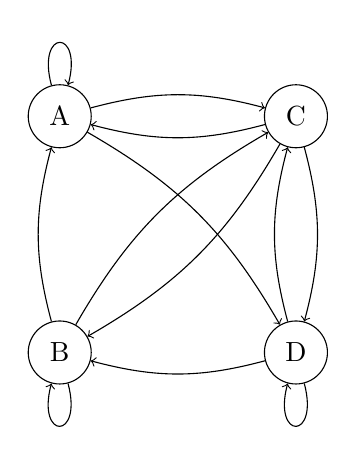
\begin{tikzpicture}[scale=1.5, node distance=2.5cm, 
                        every node/.style={circle, draw, minimum size=0.8cm},
                        every loop/.style={looseness=8}]
        % Nodes
        \node (A) at (0,2) {A};
        \node (B) at (0,0) {B};
        \node (C) at (2,2) {C};
        \node (D) at (2,0) {D};
        % Self-loops
        \path[->] (A) edge[loop above] (A);
        \path[->] (B) edge[loop below] (B);
        \path[->] (D) edge[loop below] (D);
        % Edges
        \draw[->] (A) to[bend left=15] (C);
        \draw[->] (A) to[bend left=15] (D);
        \draw[->] (B) to[bend left=15] (A);
        \draw[->] (B) to[bend left=15] (C);
        \draw[->] (C) to[bend left=15] (A);
        \draw[->] (C) to[bend left=15] (B);
        \draw[->] (C) to[bend left=15] (D);
        \draw[->] (D) to[bend left=15] (B);
        \draw[->] (D) to[bend left=15] (C);
    \end{tikzpicture}
    \end{center}
    \textbf{B:}\\
    \textbf{NO}, this is NOT an equivalence relation.\\
    \textbf{Reflexive:} No. The relation is missing $(C,C)$. Looking at the diagonal of the matrix, position [3,3] = 0, so C is not related to itself.\\
    \textbf{Symmetric:} No. We have $(A,D) \in R$ (matrix entry [1,4] = 1) but $(D,A) \notin R$ (matrix entry [4,1] = 0), thus the relation fails symmetry due to the $(A,D)$ counterexample.\\
    Since the relation fails both reflexivity and symmetry, it cannot be an equivalence relation.
\end{solution}

\question[4] Draw the Hasse diagram for divisibility on the set $\{2, 3, 4, 6, 7, 8, 12, 15\}$.

\begin{solution}
    Enter your solution here:\\
    \begin{center}
    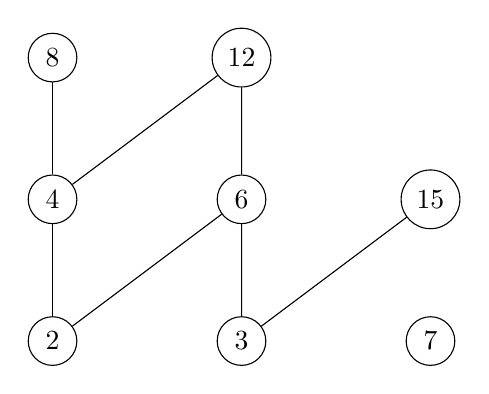
\begin{tikzpicture}[scale=1.2]
        % Bottom level
        \node[circle,draw] (2) at (0,0) {2};
        \node[circle,draw] (3) at (2,0) {3};
        \node[circle,draw] (7) at (4,0) {7};
        % Level 2
        \node[circle,draw] (4) at (0,1.5) {4};
        \node[circle,draw] (6) at (2,1.5) {6};
        \node[circle,draw] (15) at (4,1.5) {15};
        % Level 3
        \node[circle,draw] (8) at (0,3) {8};
        \node[circle,draw] (12) at (2,3) {12};
        % Edges
        \draw (2) -- (4);
        \draw (2) -- (6);
        \draw (3) -- (6);
        \draw (3) -- (15);
        \draw (4) -- (8);
        \draw (4) -- (12);
        \draw (6) -- (12);
    \end{tikzpicture}
    \end{center}
\end{solution}

\question[4] Draw the Hasse diagram for divisibility on the set $\{3, 5, 9, 11, 15, 24, 45, 135\}$.

\begin{solution}
    Enter your solution here:\\
    \begin{center}
    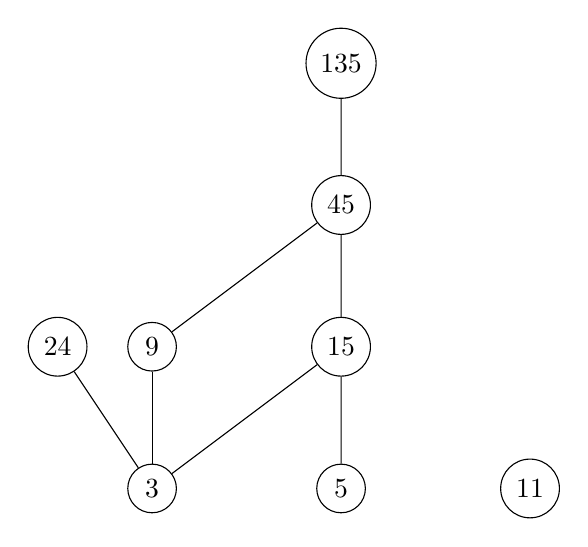
\begin{tikzpicture}[scale=1.2]
        % Bottom level
        \node[circle,draw] (3) at (0,0) {3};
        \node[circle,draw] (5) at (2,0) {5};
        \node[circle,draw] (11) at (4,0) {11};
        % Level 2
        \node[circle,draw] (9) at (0,1.5) {9};
        \node[circle,draw] (15) at (2,1.5) {15};
        \node[circle,draw] (24) at (-1,1.5) {24};
        % Level 3
        \node[circle,draw] (45) at (2,3) {45};
        % Level 4
        \node[circle,draw] (135) at (2,4.5) {135};
        % Edges
        \draw (3) -- (9);
        \draw (3) -- (15);
        \draw (3) -- (24);
        \draw (5) -- (15);
        \draw (9) -- (45);
        \draw (15) -- (45);
        \draw (45) -- (135);
    \end{tikzpicture}
    \end{center}
\end{solution}

\question[4] Draw the Hasse diagram for divisibility on the set $(\{2, 3, 4, 5, 10, 30, 33, 120\}, |)$.

\begin{solution}
    Enter your solution here:\\
    \begin{center}
    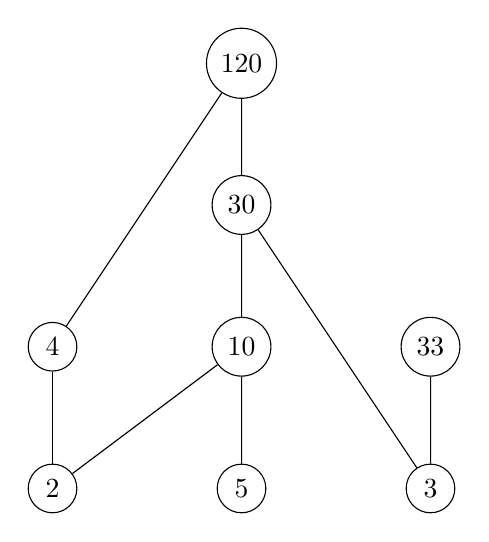
\begin{tikzpicture}[scale=1.2]
        % Bottom level
        \node[circle,draw] (2) at (0,0) {2};
        \node[circle,draw] (3) at (4,0) {3};
        \node[circle,draw] (5) at (2,0) {5};
        % Level 2
        \node[circle,draw] (4) at (0,1.5) {4};
        \node[circle,draw] (10) at (2,1.5) {10};
        \node[circle,draw] (33) at (4,1.5) {33};
        % Level 3
        \node[circle,draw] (30) at (2,3) {30};
        % Level 4
        \node[circle,draw] (120) at (2,4.5) {120};
        % Edges
        \draw (2) -- (4);
        \draw (2) -- (10);
        \draw (3) -- (30);
        \draw (3) -- (33);
        \draw (5) -- (10);
        \draw (4) -- (120);
        \draw (10) -- (30);
        \draw (30) -- (120);
    \end{tikzpicture}
    \end{center}
\end{solution}

\question[16] Answer these questions for the poset $\{3, 5, 9, 11, 15, 24, 45, 135\}$.\textbf{Hint:} Use your Hasse diagram from question 8.

\begin{parts}
\part Find the maximal elements.
\part Find the minimal elements.
\part Is there a greatest element?
\part Is there a least element?
\part Find all upper bounds of $\{3, 5\}$.
\part Find the least upper bound of $\{3, 5\}$, if it exists.
\part Find all lower bounds of $\{15, 135\}$.
\part Find the greatest lower bound of $\{15, 135\}$, if it exists.
\end{parts} 

\begin{solution}
    Enter your solution here:\\
    \textbf{A:} 11, 24, 135\\
    \textbf{B:} 3, 5, 11\\
    \textbf{C:}There is not since there is multiple maximal elements.\\
    \textbf{D:}There is not since there is multiple minimal elements.\\
    \textbf{E:} 15, 45, 135\\
    \textbf{F:} 15\\
    \textbf{G:} 3, 5, 15\\
    \textbf{H:} 15\\
\end{solution}

\question[16] Answer these questions for the poset $(\{2, 3, 4, 5, 10, 30, 33, 120\}, |)$. \textbf{Hint:} Use your Hasse diagram from question 9.

\begin{parts}
\part Find the maximal elements.
\part Find the minimal elements.
\part Is there a greatest element?
\part Is there a least element?
\part Find all upper bounds of $\{2, 5\}$.
\part Find the least upper bound of $\{2, 5\}$, if it exists.
\part Find all lower bounds of $\{30, 120\}$.
\part Find the greatest lower bound of $\{30, 120\}$, if it exists.
\end{parts} 

\begin{solution}
    Enter your solution here:\\
    \textbf{A:} 33, 120\\
    \textbf{B:} 2, 3, 5\\
    \textbf{C:}There is not since there is multiple maximal elements.\\
    \textbf{D:}There is not since there is multiple minimal elements.\\
    \textbf{E:} 10, 30, 120\\
    \textbf{F:} 10\\
    \textbf{G:} 2, 3, 5, 10, 30\\
    \textbf{H:} 30\\
\end{solution}

\question[4] Find a compatible total order using topological sorting for the divisibility relation on the set $\{1, 2, 3, 6, 10, 12, 20, 32, 40, 49.\}$.

\begin{solution}
    Enter your solution here:\\
    A possible total order from topological sorting is (1, 49, 2, 3, 32, 10, 6, 20, 40, 12).
\end{solution}
\end{questions}
\end{document}